\documentclass{article}
\usepackage[margin=1in]{geometry}
\usepackage{amsmath,amsfonts,amssymb}
\usepackage{listings}
\usepackage{color}
\usepackage{graphicx}
\usepackage{subfig}
\usepackage{blkarray}
\usepackage{multirow}
\usepackage{float}
\usepackage{caption}
\usepackage{subcaption}
\captionsetup[sub]{}

\definecolor{dkgreen}{rgb}{0,0.6,0}
\definecolor{gray}{rgb}{0.5,0.5,0.5}
\definecolor{mauve}{rgb}{0.58,0,0.82}

\newcommand\tab[1][1cm]{\hspace*{#1}}
\begin{document}
\begin{titlepage}
	\setlength{\parindent}{0pt}
	\large

\vspace*{-2cm}


\lstset{frame=tb,
  language=Python,
  aboveskip=3mm,
  belowskip=3mm,
  showstringspaces=false,
  columns=flexible,
  basicstyle={\small\ttfamily},
  numbers=none,
  numberstyle=\tiny\color{gray},
  keywordstyle=\color{blue},
  commentstyle=\color{dkgreen},
  stringstyle=\color{mauve},
  breaklines=true,
  breakatwhitespace=true,
  tabsize=3
}

University of Waterloo \par
CS 486 \par
\vspace{0.05cm}
r2knowle: 2023-10-1
\vspace{0.2cm}

{\huge Assignment \# 1 \par}
\hrule

\vspace{0.5cm}
\textbf{Q1a)} We will expand the nodes in the following order:
\[ s -> h -> k -> c -> a -> b -> d -> m -> e -> n -> g \]
Thus arriving from s to g.\\\\
\textbf{Q1bi)} This heuristic is admissible, to prove that this is the case we will use contradiction. Assume that the heuristic is not admissible this means that for some node n:
\[ h(n) > h^*(n) \]
where $h^*(n)$ is the true cost of node n. This means that the true cost of n is actually shorter with a barrier, and since a barrier only every reduces the path size this is impossible. Therefore the heuristic is admissible. \\\\
\textbf{Q1bi)} Using depth first search with this heuristic gives us the nodes expanded in the following order: \\
\[ s -> h -> k -> c -> a -> b -> d -> m -> g \]
Which gets us from s to g. \\\\
\textbf{Q1bii)} Using $A^*$ gives us the nodes expanded in the following order:  \\
\[ s -> h -> k -> f -> p -> q -> a -> r -> t -> g \]
Which gets us from s to g.\\\\\\\\
\textbf{Q2a)} Yes, in the event that all the paths have an equal cost. To prove this lets use contradiction, assume that breath width search does not expand values in the same state as uniform-cost  search does. That would imply that the node n's ancestors would be different in uniform search then breath first search. However if the ancestors are different then that would imply that breath first search is on an unoptimised path which is impossible as breath first search minimizes the number of nodes visited and since the path cost is constant this should minimize cost. Therefore because we have a contradiction breath width search is a special case of uniform-cost search.\\\\
\textbf{Q2b)} No, as there is no heuristic which guarantees us to always expand the child node (branch) consider the example in 1, we cant define a heuristic such that we will only expand the child node. \\\\
\textbf{Q2c)} Yes in the event that the heuristic function is 0, A* will preform exactly the same as uniform cost. This is because the cost of each node in A* is its uniform search cost plus the heuristic and therefore if the heuristic is zero they will be the same. 
\newpage
\textbf{Q3a)} We can represent the TSP by the following problem representation:
\begin{align*}
\textbf{States} &= \text{any combination of citites, where no city is repeated twice.} \\
\textbf{Representation} &= \text{we can represent each state by the letter of the city in the order}\\
& \text{they are visited.} \\
\textbf{Inital State} &= \text{the inital state is always city A.} \\
\textbf{Goal State} &= \text{The goal state is when all the cities are visited, cost minimized.} \\
\textbf{Sucessor Function} &= \text{The sucessor function is to move to a new state, where a new city} \\
& \text{letter is added to the end of our current state i.e we visit a new city.} \\
\textbf{Cost Function} &= \text{The cost between any state is the minimum eucliean distance } \\
& \text{ between all the cities they have in common and the one city they have}\\
& \text{different. The total cost of any state is the total eucledian distance between} \\
& \text{all the neighbouring cities in the representation.}
\end{align*}\\
\textbf{Q3b)} We can have 3 of the following heuristics: \\\\
\tab h1(n): For this heuristic the cost for any city is equal to the minimum distance from this city to any other city that we have. This is admissible as the true cost of any node will always be greater then or equal to the minimum distance, if the true cost is less than it would imply that there is a new minimum path and is thus a contradiction. \\\\
\tab h2(n): For this heuristic the cost for any city is equal to 0. This is always admissible as the actual cost of adding a city must be greater then 0. This heuristic will turn our A* algorithm into a uniform search algorithm. \\\\
\tab h3(n): the cost for this city is equal to the distance from the current city. This ensures that we will always pick the city that is cheapest from our current node to the next node. This is admissible as  there is no path that is cheaper between our current node and the next node as if there was we would use this node instead. \\\\
We should expect that h2 will get dominated by both h3 and h1, as h2 will not get rid of any states. For h3 we expect that it should dominate h1 as the actual smallest to our current node should cause a lot less errors then the entire graphs smallest.
\newpage
\textbf{Q3c)} On average (across all 10 instances of each city) we expect that each of the heuristics expand the following number of nodes for each of the cities:
\[
\begin{tabular}{l|l|c|c|c|c|c|c|c|c|c|c|c|}
\multicolumn{3}{c}{}&\multicolumn{9}{c}{Number of Cities}&\multicolumn{1}{c}{}\\
\cline{3-13}
\multicolumn{2}{c|}{}&1&2&3&4&5&6&7&8&9&10&11 \\
\cline{2-13}
\multirow{3}{*}{Heuristic}& h1 & $1$ & $1$ & $1$ & $3.6$ & $12.3$ & $52.6$ & $206.6$ & $941.3$ & $5002.8$ & $15719.7$ & $123394.6$\\
\cline{2-13}
& h2 & $1$ & $1$ & $1$ & $4$ & $15.4$ & $57.4$ & $225.9$ & $1053.6$ & $5832.2$ & $18735.1$ & $114533.8$\\
\cline{2-13}
& h3 & $1$ & $1$ & $1$ & $3.2$ & $10.2$ & $36.7$ & $138.1$ & $497.5$ & $2668.7$ & $8452.2$ & $8452.2$\\
\cline{2-13}
\end{tabular}\] \\
\[
\begin{tabular}{l|l|c|c|c|c|c|c|c|c|c|c|c|}
\multicolumn{2}{c}{}&\multicolumn{5}{c}{Number of Cities}&\multicolumn{1}{c}{}\\
\cline{3-7}
\multicolumn{2}{c|}{}&12&13 & 14 & 15 & 16 \\
\cline{2-7}
\multirow{3}{*}{Heuristic}& h1 & $343869.6$ & $1982604.5$ & $...$ & $...$ & $...$\\
\cline{2-7}
& h2 & $418689.3$ & $2020802.0$ & $...$ & $...$ & $...$ \\
\cline{2-7}
& h3 & $203459.1$ & $918482.0$ & $4323873$ & $9521119$ & $21013284$ \\
\cline{2-7}
\end{tabular}\] \\\\
Note that for h1 and h2, due to their slow nature it would take way too long to calculate for all 16 cities. Therefore as per the piazza post we only calucated the time it would take for the fastest heuristic (h3). Taking the log of these results we can then graph them to get the following graph shown on the left. By doing simple linear regression we can also predict the results for how many nodes would need to be expanded for up to the 32nd city which is seen on the right:

\begin{figure}[H]
    \centering
{{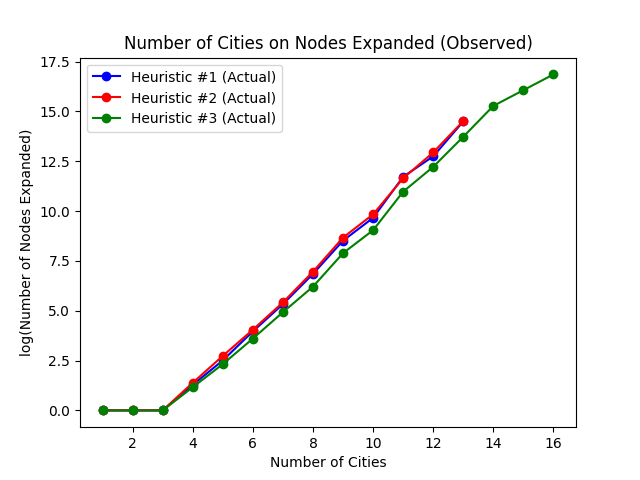
\includegraphics[width=7cm]{q1Actual.png} }}%
    \qquad
{{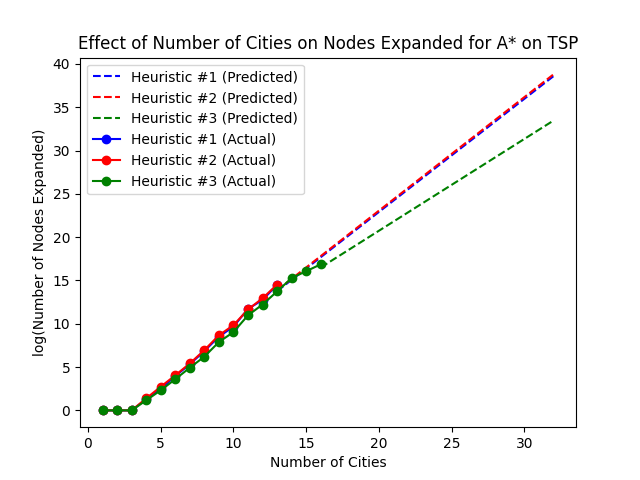
\includegraphics[width=7cm]{q1Pred.png} }}%
\end{figure}

From the graph is evident that our 3rd heuristic dominates the 1st and second heuristic. Even with the relative decrease in number of nodes expanded, this heuristic would still be incredibly slow for TSP on 32 cities, infact each of the heuristics would need to expand the following number of nodes:
\begin{align*}
\text{Heuristic \#1}:& \text{  }5.6741249252×10^{16} \text{ nodes expanded} \\
\text{Heuristic \#2}:& \text{  }6.9782360677×10^{16} \text{ nodes expanded} \\
\text{Heuristic \#3}:& \text{  }2.0486679187×10^{14} \text{ nodes expanded}
\end{align*}
Thus it would appear out of all our heuristics h3 preforms the best, as seen by the graph and the predicted number of nodes to solve the 32 city problem.
\newpage
\textbf{Code for Q3)} Here is all the code for my question 3, I exported the results to a separate python file which plotted everything in pyplot (which is not included in the below code): \\
\begin{lstlisting}
import numpy as np
import heapq


cityMap = {}                                                  # Store position of each city
stateCostMap = {}                                             # Store total cost of each state
cityMinCost = {}                                              # Store minimum cost of each city

states = []                                                   # Stores our states to expand
citiesToVisit = []                                            # Stores the cities we haven't visited

# This function takes in two city and calculates the distance between them (l2 norm)
def calculateCost(city1, city2):
    city1cords = cityMap[city1]
    city2cords = cityMap[city2]

    return np.sqrt((city1cords[0] - city2cords[0]) ** 2 + (city1cords[1] - city2cords[1]) ** 2)


# This is the third heuristic, the cost of the state + the distance to each possible next city
def getCost3(state):
    return calculateCost(state[-2], state[-1]) + stateCostMap[state[0:-1]]

# This is the second heuristic, the cost of the state + 0
def getCost2(state):
    return stateCostMap[state[0:-1]]

# This is the first heuristic, the cost of the state + the minimum distance to the current state
def getCost1(state):
    return cityMinCost[city] + stateCostMap[state[0:-1]]


# db refers to the number of cities we need to loop through
for db in range(2, 14):
    numberOfStates = 0                                            # Stores total states for problem set
    for instance in range(1, 11):

        # Empty out our global variables
        cityMap = {}
        stateCostMap = {}
        cityMinCost = {}
        states = []
        citiesToVisit = []

        # Read in the file
        file = open("randTSP/" + str(db) + "/instance_" + str(instance) + ".txt", "r")
        numberOfCities = int(file.readline())

        states = []
        heapq.heapify(states)                                     # States is a heap so we do our operations quickly
        finalGoalString = []

        # Convert the points in the text file into our dictionaries
        for i in range(0, numberOfCities):
            line = file.readline().split(" ")
            line[2] = line[2].split('\n')[0]

            if line[0] == 'A':
                stateCostMap['A'] = 0
            else:
                citiesToVisit.append(line[0])
            finalGoalString.append(line[0])
            cityMap[line[0]] = (int(line[1]), int(line[2]))

        listOfAllCites = citiesToVisit + ["A"]

        # Manually calculate the children from the first node
        for cityRef in citiesToVisit:
            minSize = -1
            for city in listOfAllCites:
                if (cityRef != city):
                    currSize = calculateCost(city, cityRef)
                    if (minSize == -1 or minSize > currSize):
                        minSize = currSize
            cityMinCost[cityRef] = minSize

        for city in citiesToVisit:
            newState = "A" + city
            # Add the distance + state representation onto the heap for later
            heapq.heappush(states, (getCost3(newState), newState))

        while True:
            numberOfStates += 1

            # Pop the closest state
            curPick = heapq.heappop(states)[1]

            count = 0
            # Add its children to the heap
            for city in citiesToVisit:
                if city not in curPick:
                    actualCost = calculateCost(curPick[-1], city)
                    stateCostMap[curPick] = actualCost + stateCostMap[curPick[0:-1]]
                    newState = curPick + city
                    heapq.heappush(states, (getCost3(newState), newState))
                    count += 1

            if count <= 1:
                break

    print("City " + str(db) +"#: " +str(numberOfStates/10))
\end{lstlisting}
\newpage
\textbf{Q4a)} To begin we can define Sudoku as a CSP. Thus we will be having the following terms:
\begin{align*}
\textbf{Variables}: & \text{ x = \{1,...,9\} and y = \{1,...,9\}. We will have x represent the current row} \\
&\text{ and y represent the current column. Thus an element can be represented} \\
&\text{ as }G_{x,y}  \\
\textbf{Domain}: & \text{ Each } G_{x,y} \text{ will belong to \{1,2,3,4,5,6,7,8,9\} } \\
\textbf{Constraints}: & \text{ } \forall x \in \{1,..,9\} \text{ and } \forall y \in \{1,..,9\} \text{ where } x \neq y, \forall i \in \{1,..,9\} \text{ } G_{i,x} \neq G_{i,y} \\
& \text{ } \forall x \in \{1,..,9\} \text{ and } \forall y \in \{1,..,9\} \text{ where } x \neq y, \forall i \in \{1,..,9\} \text{ } G_{x,i} \neq G_{y,i} \\
& \text{ } \forall i1 \in \{1,2,3\}, \forall i2 \in \{1,2,3\} \text{ and } \forall x = \{1,2,3\} \text { and } \forall y = \{1,2,3\}: \\
& \hspace{0.5cm} G_{[i1\times x, i2 \times y]} = \{1,2,3,4,5,6,7,8,9\}
\end{align*}
These three constraints represent the each value being unique along the row and column. Moreover each 3x3 cube needs to have exactly $\{1,2,3,4,5,6,7,8,9\}$ with no repeats. \\\\
\textbf{Q4b)} We have the following solutions for the problems:

\begin{figure}[H]
\begin{minipage}[c]{0.45\linewidth}
\centering
\begin{tabular}{ |ccc|ccc|ccc| } 
\hline
 6 & 1 & 2 & 9 & 8 & 4 & 7 & 5 & 3 \\ 
 9 & 4 & 5 & 3 & 2 & 7 & 6 & 8 & 1 \\ 
 3 & 7 & 8 & 6 & 5 & 1 & 9 & 2 & 4 \\ 
\hline
 5 & 9 & 1 & 2 & 7 & 6 & 3 & 4 & 8 \\
 7 & 6 & 3 & 8 & 4 & 5 & 2 & 1 & 9 \\
 8 & 2 & 4 & 1 & 3 & 9 & 5 & 6 & 7 \\
\hline
 2 & 3 & 9 & 5 & 1 & 8 & 4 & 7 & 6 \\
 1 & 5 & 7 & 4 & 6 & 3 & 8 & 9 & 2 \\
 4 & 8 & 6 & 7 & 9 & 2 & 1 & 3 & 5 \\
\hline
\end{tabular}
\caption{Easy Sudoku}
\end{minipage}
\hfill
\begin{minipage}[c]{0.45\linewidth}
\centering
\begin{tabular}{ |ccc|ccc|ccc| } 
\hline
 3 & 4 & 8 & 1 & 6 & 7 & 9 & 2 & 5 \\
 6 & 5 & 7 & 3 & 9 & 2 & 1 & 8 & 4 \\
 2 & 1 & 9 & 5 & 8 & 4 & 3 & 7 & 6 \\
\hline
 7 & 8 & 1 & 2 & 3 & 6 & 4 & 5 & 9 \\
 4 & 2 & 5 & 7 & 1 & 9 & 6 & 3 & 8 \\
 9 & 3 & 6 & 4 & 5 & 8 & 2 & 1 & 7 \\
\hline
 1 & 9 & 3 & 6 & 7 & 5 & 8 & 4 & 2 \\
 5 & 6 & 2 & 8 & 4 & 1 & 7 & 9 & 3 \\
 8 & 7 & 4 & 9 & 2 & 3 & 5 & 6 & 1 \\
\hline
\end{tabular}
\caption{Medium Sudoku}
\end{minipage}%
\hfill
\begin{minipage}[c]{0.45\linewidth}
\centering
\begin{tabular}{ |ccc|ccc|ccc| } 
\hline
 1 & 6 & 3 & 9 & 2 & 5 & 4 & 7 & 8 \\
 8 & 9 & 4 & 3 & 6 & 7 & 5 & 1 & 2 \\
 7 & 5 & 2 & 4 & 8 & 1 & 6 & 3 & 9 \\
\hline
 2 & 1 & 6 & 7 & 4 & 9 & 3 & 8 & 5 \\
 3 & 7 & 9 & 6 & 5 & 8 & 2 & 4 & 1 \\
 5 & 4 & 8 & 2 & 1 & 3 & 9 & 6 & 7 \\
\hline
 6 & 3 & 5 & 1 & 7 & 2 & 8 & 9 & 4 \\
 9 & 2 & 1 & 8 & 3 & 4 & 7 & 5 & 6 \\
 4 & 8 & 7 & 5 & 9 & 6 & 1 & 2 & 3 \\
\hline
\end{tabular}
\caption{Hard Sudoku}
\end{minipage}
\hfill
\begin{minipage}[c]{0.45\linewidth}
\centering
\begin{tabular}{ |ccc|ccc|ccc| } 
\hline
 3 & 4 & 1 & 9 & 7 & 8 & 6 & 5 & 2 \\
 5 & 9 & 2 & 1 & 6 & 3 & 7 & 4 & 8 \\
 7 & 6 & 8 & 4 & 5 & 2 & 3 & 9 & 1 \\
\hline
 6 & 1 & 9 & 8 & 2 & 7 & 4 & 3 & 5 \\
 8 & 2 & 3 & 5 & 9 & 4 & 1 & 7 & 6 \\
 4 & 5 & 7 & 6 & 3 & 1 & 8 & 2 & 9 \\
\hline
 9 & 3 & 6 & 7 & 1 & 5 & 2 & 8 & 4 \\
 2 & 8 & 5 & 3 & 4 & 6 & 9 & 1 & 7 \\
 1 & 7 & 4 & 2 & 8 & 9 & 5 & 6 & 3 \\
\hline
\end{tabular}
\caption{Evil Sudoku}
\end{minipage}%
\end{figure} 
On the next page will be the timings and the discussion of the different methods of solving for Sudoku.
\newpage
\textbf{Q4c)} Below in the tables for the preformance of the different version we used. Note that the means and standard deviation for both the nodes and timings are in their own tables:


\begin{figure}[H]
\begin{minipage}[c]{0.9\linewidth}
\centering
\begin{tabular}{ |c||c|c|c|c| } 
\hline
\text{ } & \text{Easy Sudoku} & \text{Medium Sudoku} & \text{Hard Sudoku} & \text{Evil Sodoku} \\
\hline
\hline
\text{Version A} & 0.263372 & 18.2829 & 230.562 & 2033.96\\
\text{Version B} & 0.015204 & 0.08212 & 5.02846 & 5.35182 \\
\text{Version C} & 0.014104 & 0.01438 & 0.01531 & 0.02358\\
\hline
\end{tabular}
\caption{Mean Run Time (Seconds)}
\end{minipage}
\hfill
\vspace{0.5cm}
\begin{minipage}[c]{0.9\linewidth}
\centering
\begin{tabular}{ |c||c|c|c|c| } 
\hline
\text{ } & \text{Easy Sudoku} & \text{Medium Sudoku} & \text{Hard Sudoku} & \text{Evil Sodoku} \\
\hline
\hline
\text{Version A} & 0.578759 & 23.8846 & 91.9113 & 1860.95\\
\text{Version B} & 0.007715 & 0.11744 & 8.68887 & 11.3717\\
\text{Version C} & 0.008285 & 0.00104 & 0.00809 & 0.13266\\
\hline
\end{tabular}
\caption{Standard Deviation for Run Time (Seconds)}
\end{minipage}%
\hfill
\vspace{0.5cm}
\begin{minipage}[c]{0.9\linewidth}
\centering
\begin{tabular}{ |c||c|c|c|c| } 
\hline
\text{ } & \text{Easy Sudoku} & \text{Medium Sudoku} & \text{Hard Sudoku} & \text{Evil Sodoku} \\
\hline
\hline
\text{Version A} & 197364 & $1.29661\times 10^7$ &  $2.30562\times 10^8$ & $1.51687 \times 10^9$\\
\text{Version B} & 696.74 & 22904.7 & $1.77178\times 10^{6}$& $1.83571 \times 10^{6}$ \\
\text{Version C} & 67.58 & 213.54 & 83.56 & 635.96\\
\hline
\end{tabular}
\caption{Mean Nodes Expanded}
\end{minipage}
\hfill
\vspace{0.5cm}
\begin{minipage}[c]{0.9\linewidth}
\centering
\begin{tabular}{ |c||c|c|c|c| } 
\hline
\text{ } & \text{Easy Sudoku} & \text{Medium Sudoku} & \text{Hard Sudoku} & \text{Evil Sodoku} \\
\hline
\hline
\text{Version A} & 434741 & $2.38846\times 10^7$ &  $9.19113\times 10^7$ & $1.38905 \times 10^9$\\
\text{Version B} & 578.016 & 37394.4 & $3.10042 \times 10^{6}$ & $3.92013 \times 10^{6}$ \\
\text{Version C} & 8.25 & 24.3329 & 3.5 & 88.357\\
\hline
\end{tabular}
\caption{Standard Deviation for Mean Nodes Expanded}
\end{minipage}%
\end{figure} 
From these results we can observe that version C and version B do far better then version A. This is because the runtime is directly tied to the number of nodes that we need to expand, and version A will expand the most nodes as it only terminates when it cant find any values in the domain to satisfy a variable. On the otherhand version B and version C can look ahead and see which variables will be impossible to satisfy and can avoid going all the way to the leaf before terminating.\\\\
	Version C differs from version B as it uses 3 heuristics in order to improve its run time:
	\begin{align*}
\text{Heuristic \#1}:& \text{ Expand the most constrained variable first } \\
\text{Heuristic \#2}:& \text{ Use the least constraining values from the domain }\\
\text{Heuristic \#3}:& \text{ Expand the most constraing variable  }
\end{align*}
In this order we will expand the variables, which as we saw decreased the run time and the number of nodes needed to expand from version B. All the code for each of the versions is provided on the following pages.
\newpage
\textbf{Code for Version A)}
\lstset{frame=tb,
  language=C,
  aboveskip=3mm,
  belowskip=3mm,
  showstringspaces=false,
  columns=flexible,
  basicstyle={\small\ttfamily},
  numbers=none,
  numberstyle=\tiny\color{gray},
  keywordstyle=\color{blue},
  commentstyle=\color{dkgreen},
  stringstyle=\color{mauve},
  breaklines=true,
  breakatwhitespace=true,
  tabsize=3
}
\begin{lstlisting}
#include <iostream>
#include <string>
#include <chrono>
#include <vector>
#include <random>
#include <algorithm>
#include <numeric>

using namespace std::chrono;
using namespace std;

// Store the boards as strings
std::string easyBoard  =  "010900053040300681070050900590070040700805009020030067009010070157003090480002030";
std::string mediumBoard = "000160925007000180000080006780200000025010630000008017100070000062000700874023000";
std::string hardBoard =   "103005400800000000000080600006049000079608240000210900005070000000000006007500103";
std::string evilBoard =   "001970000090003008000402000610000405003000100407000029000705000200300010000089500";

// This counter will be used to keep track of the number of nodes expanded
int nodesExpanded = 0;


// Helper function to display the grid
void printGrid(const int map[81]) {
    for (int i = 0; i < 9; i++) {
        cout << "{";
        for (int x = 0; x<9; x++) {
            cout << map[i*9+x];
            if (x != 8) {
                cout << ", ";
            }
        }
        cout << "}," << endl;
    }
}


/*
 * This function is used to set the domain, the domain stores all the possible values at each index.
 *  Each time we add a value we need to update the domain accordingly, thus we take in the index we
 *  want to change
 */
bool setDomain(int map[81], int domain[][10], int idx) {
    int row = idx/9;
    int column = idx%9;

    for ( int i = 0; i < 9; i++ ) {
        domain[i+row*9][map[idx]] = 1;              // Update along the row
        domain[i*9 +column][map[idx]] = 1;          // Update along the column
    }

    int rowStart = row/3;                           // Start position of grid (row)
    int columnStart = column/3;                     // Start position of grid (column)

    for (int x = 0; x < 3; x++) {
        for (int y = 0; y < 3; y++) {
            domain[columnStart*3 + (y+rowStart*3)*9 + x][map[idx]] = 1;
        }
    }
    return true;


}



/* We treat the original array like doing n insert, where n
 *  is the number of non zero elements in our array
 */
void init(int map[81], int takenValues[][10]) {
    for ( int y = 0; y < 9 ; y++ ) {
        for ( int x = 0; x < 9 ; x++ ) {
            if ( map[y*9+x] != 0 ) {
                setDomain(map, takenValues, y*9+x);
            }
        }
    }

}

/*
 * This is the main method for solving any sukodku problem, to begin we will pick a random
 *  index to loop through, after this we will we will check if there are any more values to read
 *  in. After this we will check our domain for that variable, and continue if theres a valid placement.
 *  We continue until we get a solution
 */
bool sukodku(const int board[81], const int domain[][10], const vector<int>* const valsToReplace, int pos) {

    int positionToCheck = valsToReplace->operator[](pos);
    pos++;

    if (valsToReplace->size() < pos) {
        printGrid(board);                   // Print the solution!
        return true;
    }

    for (int idx = 1; idx < 10; idx++) {

        if (domain[positionToCheck][idx] != 1) { // Check if the domain is empty

            nodesExpanded++;                     // Expand the nodes


            int newDomain[81][10];               // Make a deep copy of the domain
            int newMap[81];                      // Make a deep copy of the matrix

            for (int i = 0; i < 81; i++) {
                newMap[i] = board[i];
                for (int x = 0; x < 10; x++) {
                    newDomain[i][x] = domain[i][x];
                }
            }

            newMap[positionToCheck] = idx;
            setDomain(newMap, newDomain, positionToCheck);

            // Recurse until we can find the proper solution
            bool result = sukodku(newMap, newDomain, valsToReplace, pos);

            if (result) {
                return true;
            }
        }
    }

    return false;
}
int main() {

    vector<int> timings;                             // Vector for storing the timings per run
    vector<int> nodes;                               // Vector for storing the number of nodes per run

    auto rng = std::default_random_engine{};         // Random needed for shuffle
    rng.seed(getpid());

    for (int runs = 0; runs < 50 ; runs++ ) {         // Number of runs to do

        std::string readin = evilBoard;              // Which board to use

        // This will convert the string into a 1D int array
        int board[81];
        for (int y = 0; y < 9; y++) {
            for (int x = 0; x < 9; x++) {
                board[y * 9 + x] = readin[y * 9 + x] - '0';
            }
        }

        int takenValues[81][10];

        for (int i = 0; i < 81; i++) {
            for (int x = 0; x < 10; x++) {
                takenValues[i][x] = 0;
            }
        }

        init(board, takenValues);
        // This will store all the indexes where we have a zero
        vector<int> valsToReplace;

        for (int i = 0; i < 81; i++) {
            if (board[i] == 0) {
                valsToReplace.push_back(i);
            }
        }

        // Shuffle the list of positions to check
        shuffle(valsToReplace.begin(), valsToReplace.end(), rng);

        nodesExpanded = 0;
        // Start the time
        auto start = high_resolution_clock::now();

        sukodku(board, takenValues, &valsToReplace, 0);
        // Finish the time
        auto stop = high_resolution_clock::now();

        auto duration = duration_cast<microseconds>(stop - start);

        timings.push_back(duration.count());
        nodes.push_back(nodesExpanded);

        std::cout << runs << endl;
    }


    // The below code will calculate the timiing and number of nodes for each run
    double sum = std::accumulate(timings.begin(), timings.end(), 0.0);
    double mean = sum / timings.size();

    double var = 0;
    for( int n = 0; n < timings.size(); n++ )
    {
        var += (timings[n] - mean) * (timings[n] - mean);
    }
    var /= timings.size();
    double stdev = sqrt(var);

    std::cout << "Timing average: " << mean << " | Timing std deviation: " << stdev << endl;

    sum = std::accumulate(nodes.begin(), nodes.end(), 0.0);
    mean = sum / nodes.size();



    var = 0;
    for( int n = 0; n < nodes.size(); n++ )
    {
        var += (nodes[n] - mean) * (nodes[n] - mean);
    }
    var /= nodes.size();
    stdev = sqrt(var);

    std::cout << "Node average: " << mean << " | Node std deviation: " << stdev << endl;

    return 0;
}
\end{lstlisting}
\newpage
\textbf{Code for Version B)}
\begin{lstlisting}
#include <iostream>
#include <string>
#include <chrono>
#include <vector>
#include <random>
#include <algorithm>
#include <numeric>

using namespace std::chrono;
using namespace std;

// Store the boards as strings
std::string easyBoard  =  "010900053040300681070050900590070040700805009020030067009010070157003090480002030";
std::string mediumBoard = "000160925007000180000080006780200000025010630000008017100070000062000700874023000";
std::string hardBoard =   "103005400800000000000080600006049000079608240000210900005070000000000006007500103";
std::string evilBoard =   "001970000090003008000402000610000405003000100407000029000705000200300010000089500";

std::string debug     =   "004678912672195348198342567859761423426853791713924856961537284287419635345286179";


// This counter will be used to keep track of the number of nodes expanded
int nodesExpanded = 0;


// Helper function to display the grid
void printGrid(const int map[81]) {
    for (int i = 0; i < 9; i++) {
        cout << "{";
        for (int x = 0; x<9; x++) {
            cout << map[i*9+x];
            if (x != 8) {
                cout << ", ";
            }
        }
        cout << "}," << endl;
    }
}


/*
 * This function is used to set the domain, the domain stores all the possible values at each index.
 *  Each time we add a value we need to update the domain accordingly, thus we take in the index we
 *  want to change
 */
bool setDomain(int map[81], int domain[][10], int idx) {
    int row = idx/9;
    int column = idx%9;

    for ( int i = 0; i < 9; i++ ) {
        domain[i+row*9][map[idx]] = 1;              // Update along the row
        domain[i*9 +column][map[idx]] = 1;          // Update along the column
    }

    int rowStart = row/3;                           // Start position of grid (row)
    int columnStart = column/3;                     // Start position of grid (column)

    for (int x = 0; x < 3; x++) {
        for (int y = 0; y < 3; y++) {
            domain[columnStart*3 + (y+rowStart*3)*9 + x][map[idx]] = 1;
        }
    }
    return true;


}



/* We treat the original array like doing n insert, where n
 *  is the number of non zero elements in our array
 */
void init(int map[81], int takenValues[][10]) {
    for ( int y = 0; y < 9 ; y++ ) {
        for ( int x = 0; x < 9 ; x++ ) {
            if ( map[y*9+x] != 0 ) {
                setDomain(map, takenValues, y*9+x);
            }
        }
    }

}

/*
 * This is the main method for solving any sukodku problem, to begin we will pick a random
 *  index to loop through, after this we will we will check if there are any more values to read
 *  in. After this we will check our domain for that variable, and continue if theres a valid placement.
 *  We continue until we get a solution
 */
bool sukodku(const int board[81], const int domain[][10], const vector<int>* const valsToReplace, int pos) {

    int positionToCheck = valsToReplace->operator[](pos);
    pos++;

    if (valsToReplace->size() < pos) {
        printGrid(board);                   // Print the solution!
        return true;
    }

    for (int idx = 1; idx < 10; idx++) {

        if (domain[positionToCheck][idx] != 1) { // Check if the domain is empty

            nodesExpanded++;                     // Expand the nodes

            int newDomain[81][10];               // Make a deep copy of the domain
            int newMap[81];                      // Make a deep copy of the matrix

            for (int i = 0; i < 81; i++) {
                newMap[i] = board[i];
                for (int x = 0; x < 10; x++) {
                    newDomain[i][x] = domain[i][x];
                }
            }

            newMap[positionToCheck] = idx;
            setDomain(newMap, newDomain, positionToCheck);

            bool fullyUsed = true;    // store if any variable is saturated

            // This for loop will go over all the zeros and check if we fully saturated any of them
            for (int i = 0; i < 81; i++) {
                if (newMap[i] == 0) {
                    fullyUsed = true;
                    for (int x = 1; x < 10; x++) {
                        if (newDomain[i][x] == 0) { fullyUsed = false; }
                    }
                    if (fullyUsed) {
                        i += 100;
                    }
                }
            }

            if (!fullyUsed) {

                // Recurse until we can find the proper solution
                bool result = sukodku(newMap, newDomain, valsToReplace, pos);

                if (result) {
                    return true;
                }
            } else {
                // Check to see if we are at the solution which is one away form being solved
                bool hasNoZeros = true;
                for (int i : newMap) {
                    if (i == 0){
                        hasNoZeros = false;
                    }
                }

                if (hasNoZeros) {
                    // if one away from being solved run it again just to check
                    bool result = sukodku(newMap, newDomain, valsToReplace, pos);

                    if (result) {
                        return true;
                    }
                }
            }
        }
    }

    return false;
}
int main() {

    vector<int> timings;                             // Vector for storing the timings per run
    vector<int> nodes;                               // Vector for storing the number of nodes per run

    auto rng = std::default_random_engine{};         // Random needed for shuffle
    rng.seed(getpid());

    for (int runs = 0; runs < 50 ; runs++ ) {         // Number of runs to do

        std::string readin = evilBoard;              // Which board to use

        // This will convert the string into a 1D int array
        int board[81];
        for (int y = 0; y < 9; y++) {
            for (int x = 0; x < 9; x++) {
                board[y * 9 + x] = readin[y * 9 + x] - '0';
            }
        }

        int takenValues[81][10];

        for (int i = 0; i < 81; i++) {
            for (int x = 0; x < 10; x++) {
                takenValues[i][x] = 0;
            }
        }

        init(board, takenValues);
        // This will store all the indexes where we have a zero
        vector<int> valsToReplace;

        for (int i = 0; i < 81; i++) {
            if (board[i] == 0) {
                valsToReplace.push_back(i);
            }
        }

        // Shuffle the list of positions to check
        shuffle(valsToReplace.begin(), valsToReplace.end(), rng);

        nodesExpanded = 0;
        // Start the time
        auto start = high_resolution_clock::now();

        sukodku(board, takenValues, &valsToReplace, 0);
        // Finish the time
        auto stop = high_resolution_clock::now();

        auto duration = duration_cast<microseconds>(stop - start);

        timings.push_back(duration.count());
        nodes.push_back(nodesExpanded);

        std::cout << runs << endl;
    }


    // The below code will calculate the timiing and number of nodes for each run
    double sum = std::accumulate(timings.begin(), timings.end(), 0.0);
    double mean = sum / timings.size();

    double var = 0;
    for( int n = 0; n < timings.size(); n++ )
    {
        var += (timings[n] - mean) * (timings[n] - mean);
    }
    var /= timings.size();
    double stdev = sqrt(var);

    std::cout << "Timing average: " << mean << " | Timing std deviation: " << stdev << endl;

    sum = std::accumulate(nodes.begin(), nodes.end(), 0.0);
    mean = sum / nodes.size();



    var = 0;
    for( int n = 0; n < nodes.size(); n++ )
    {
        var += (nodes[n] - mean) * (nodes[n] - mean);
    }
    var /= nodes.size();
    stdev = sqrt(var);

    std::cout << "Node average: " << mean << " | Node std deviation: " << stdev << endl;

    return 0;
}
\end{lstlisting}
\textbf{Code for Version C)}
\begin{lstlisting}
#include <iostream>
#include <string>
#include <chrono>
#include <vector>
#include <random>
#include <algorithm>
#include <numeric>

using namespace std::chrono;
using namespace std;

// Store the boards as strings
std::string easyBoard  =  "010900053040300681070050900590070040700805009020030067009010070157003090480002030";
std::string mediumBoard = "000160925007000180000080006780200000025010630000008017100070000062000700874023000";
std::string hardBoard =   "103005400800000000000080600006049000079608240000210900005070000000000006007500103";
std::string evilBoard =   "001970000090003008000402000610000405003000100407000029000705000200300010000089500";

std::string debug     =   "004678912672195348198342567859761423426853791713924856961537284287419635345286179";


// This counter will be used to keep track of the number of nodes expanded
int nodesExpanded = 0;


// This will return the best variable, weight placed on constrained rather then constraining
int getBestVariable(const int domain[][10], const vector<int> *terms) {

    int maxScore = 0;
    int valToReturn = terms->at(0);

    for (int i = 0; i < 81; i++) {
        int count = 0;
        for (int x = 1; x < 10; x++) {
            if (domain[i][x] != 0) {
                count++;
            }
        }
    }

    for (auto idx : *terms) {
        // Calculations for constraints on this variable
        int constrainedAmount = 0;

        for (int x = 1; x < 10; x++) {
            if (domain[idx][x] != 0) {
                constrainedAmount += 1;
            }
        }

        // Calculations for how this variable impacts others constraints
        int constrainingAmount = 0;

        int row = idx/9;
        int column = idx%9;

        for ( int i = 0; i < 9; i++ ) {
            if (domain[i+row*9][idx] == 0) { constrainingAmount++; }
            if (domain[i*9 +column][idx] == 0) { constrainingAmount++; }
        }

        int rowStart = row/3;
        int columnStart = column/3;

        for (int x = 0; x < 3; x++) {
            for (int y = 0; y < 3; y++) {
                if (domain[columnStart*3 + (y+rowStart*3)*9 + x] != 0) {
                    constrainingAmount++;
                }
            }
        }

        // We weigh being constrained much more than constraining other variables
        if (maxScore < constrainedAmount*9 + constrainingAmount) {
            maxScore = constrainedAmount*9 + constrainingAmount;
            valToReturn = idx;
        }



    }

    return valToReturn;

}
// Helper function to display the grid
void printGrid(const int map[81]) {
    for (int i = 0; i < 9; i++) {
        cout << "{";
        for (int x = 0; x<9; x++) {
            cout << map[i*9+x];
            if (x != 8) {
                cout << ", ";
            }
        }
        cout << "}," << endl;
    }
}


/*
 * This function is used to set the domain, the domain stores all the possible values at each index.
 *  Each time we add a value we need to update the domain accordingly, thus we take in the index we
 *  want to change
 */
bool setDomain(int map[81], int domain[][10], int idx) {
    int row = idx/9;
    int column = idx%9;

    for ( int i = 0; i < 9; i++ ) {
        domain[i+row*9][map[idx]] = 1;              // Update along the row
        domain[i*9 +column][map[idx]] = 1;          // Update along the column
    }

    int rowStart = row/3;                           // Start position of grid (row)
    int columnStart = column/3;                     // Start position of grid (column)

    for (int x = 0; x < 3; x++) {
        for (int y = 0; y < 3; y++) {
            domain[columnStart*3 + (y+rowStart*3)*9 + x][map[idx]] = 1;
        }
    }
    return true;

}


// This method gets us the optimal domain for our variable
void getDomain(vector<int> *options, const int domain[][10], const int board[81], int idx) {

    vector<pair<int,int>> temp;
    int count[10];

    for (int i = 0; i < 81; i++ ) {
        if (board[i] != 0) {
            count[board[i]] += 1;
        }
    }

    for (int x = 1; x < 10; x++) {
        if (domain[idx][x] == 0) {
            temp.emplace_back(count[x], x);
        }
    }

    std::sort(temp.begin(), temp.end(), [](const auto& a, const auto& b) {
        return a.first > b.first; // Sort in descending order
    });

    for (const auto& pair : temp) {
        options->push_back(pair.second);
    }


}



/* We treat the original array like doing n insert, where n
 *  is the number of non zero elements in our array
 */
void init(int map[81], int takenValues[][10]) {
    for ( int y = 0; y < 9 ; y++ ) {
        for ( int x = 0; x < 9 ; x++ ) {
            if ( map[y*9+x] != 0 ) {
                setDomain(map, takenValues, y*9+x);
            }
        }
    }

}

/*
 * This is the main method for solving any sukodku problem, to begin we will pick a random
 *  index to loop through, after this we will we will check if there are any more values to read
 *  in. After this we will check our domain for that variable, and continue if theres a valid placement.
 *  We continue until we get a solution
 */
bool sukodku(const int board[81], const int domain[][10], const vector<int>* const valsToReplace, int pos) {

    if (valsToReplace->empty()) {
        printGrid(board);                   // Print the solution!
        return true;
    }

    int positionToCheck = getBestVariable(domain, valsToReplace);

    vector<int> newVector;
    for (int i = 0; i < valsToReplace->size(); i++) {
        if (valsToReplace->at(i) != positionToCheck) {
            newVector.push_back(valsToReplace->at(i));
        }
    }

    vector<int> valsToSort;

    // Call our method to get the best domain
    getDomain(&valsToSort, domain,board, positionToCheck);
    for (int idx : valsToSort){

        if (domain[positionToCheck][idx] != 1) { // Check if the domain is empty

            nodesExpanded++;                     // Expand the nodes

            int newDomain[81][10];               // Make a deep copy of the domain
            int newMap[81];                      // Make a deep copy of the matrix

            for (int i = 0; i < 81; i++) {
                newMap[i] = board[i];
                for (int x = 0; x < 10; x++) {
                    newDomain[i][x] = domain[i][x];
                }
            }

            newMap[positionToCheck] = idx;
            setDomain(newMap, newDomain, positionToCheck);

            bool fullyUsed = true;    // store if any variable is saturated

            // This for loop will go over all the zeros and check if we fully saturated any of them
            for (int i = 0; i < 81; i++) {
                if (newMap[i] == 0) {
                    fullyUsed = true;
                    for (int x = 1; x < 10; x++) {
                        if (newDomain[i][x] == 0) { fullyUsed = false; }
                    }
                    if (fullyUsed) {
                        i += 100;
                    }
                }
            }

            if (!fullyUsed) {

                // Recurse until we can find the proper solution
                bool result = sukodku(newMap, newDomain, &newVector, pos);

                if (result) {
                    return true;
                }
            } else {
                // Check to see if we are at the solution which is one away form being solved
                bool hasNoZeros = true;
                for (int i : newMap) {
                    if (i == 0){
                        hasNoZeros = false;
                    }
                }

                if (hasNoZeros) {
                    // if one away from being solved run it again just to check
                    bool result = sukodku(newMap, newDomain, &newVector, pos);

                    if (result) {
                        return true;
                    }
                }
            }
        }
    }

    return false;
}
int main() {

    vector<int> timings;                             // Vector for storing the timings per run
    vector<int> nodes;                               // Vector for storing the number of nodes per run

    auto rng = std::default_random_engine{};         // Random needed for shuffle
    rng.seed(getpid());

    for (int runs = 0; runs < 50 ; runs++ ) {         // Number of runs to do

        std::string readin = easyBoard;              // Which board to use

        // This will convert the string into a 1D int array
        int board[81];
        for (int y = 0; y < 9; y++) {
            for (int x = 0; x < 9; x++) {
                board[y * 9 + x] = readin[y * 9 + x] - '0';
            }
        }

        int takenValues[81][10];

        for (int i = 0; i < 81; i++) {
            for (int x = 0; x < 10; x++) {
                takenValues[i][x] = 0;
            }
        }

        init(board, takenValues);
        // This will store all the indexes where we have a zero
        vector<int> valsToReplace;

        for (int i = 0; i < 81; i++) {
            if (board[i] == 0) {
                valsToReplace.push_back(i);
            }
        }

        // Shuffle the list of positions to check
        shuffle(valsToReplace.begin(), valsToReplace.end(), rng);

        nodesExpanded = 0;
        // Start the time
        auto start = high_resolution_clock::now();

        sukodku(board, takenValues, &valsToReplace, 0);
        // Finish the time
        auto stop = high_resolution_clock::now();

        auto duration = duration_cast<microseconds>(stop - start);

        timings.push_back(duration.count());
        nodes.push_back(nodesExpanded);

        std::cout << runs << endl;
    }


    // The below code will calculate the timiing and number of nodes for each run
    double sum = std::accumulate(timings.begin(), timings.end(), 0.0);
    double mean = sum / timings.size();

    double var = 0;
    for( int n = 0; n < timings.size(); n++ )
    {
        var += (timings[n] - mean) * (timings[n] - mean);
    }
    var /= timings.size();
    double stdev = sqrt(var);

    std::cout << "Timing average: " << mean << " | Timing std deviation: " << stdev << endl;

    sum = std::accumulate(nodes.begin(), nodes.end(), 0.0);
    mean = sum / nodes.size();



    var = 0;
    for( int n = 0; n < nodes.size(); n++ )
    {
        var += (nodes[n] - mean) * (nodes[n] - mean);
    }
    var /= nodes.size();
    stdev = sqrt(var);

    std::cout << "Node average: " << mean << " | Node std deviation: " << stdev << endl;

    return 0;
}
\end{lstlisting}
\end{titlepage}
\end{document}